\chapter{Synthetic Graph Generation for Feature Isolation}

To better understand the underlying reasons for the small separators observed in road networks, we investigate the influence of specific graph properties in isolation.
This chapter details our approach to generating synthetic graph classes that exhibit selected features characteristic of road networks, such as low average degree, specific degree distributions, or properties related to planarity and locality.
By analyzing the separator sizes within these synthetic graphs, we aim to determine which properties, or combinations thereof, are crucial for enabling small separators.
We explore properties including, degree distribution, locality, planarity and hierarchical structure.

\section{Degree Distribution}

Our initial focus is on isolating the effect of the degree distribution.
Road networks are known to be sparse graphs.
The specific PTV Europe road network dataset \cite{ptv_group_dimacs-europe_2009} utilized in our experiments exhibits a average vertex degree of approximately \(2.47\).
A detailed visualization of the degree distribution for this network is provided in \cref{fig:degree_dist_europe}.

\begin{figure}
    \centering
    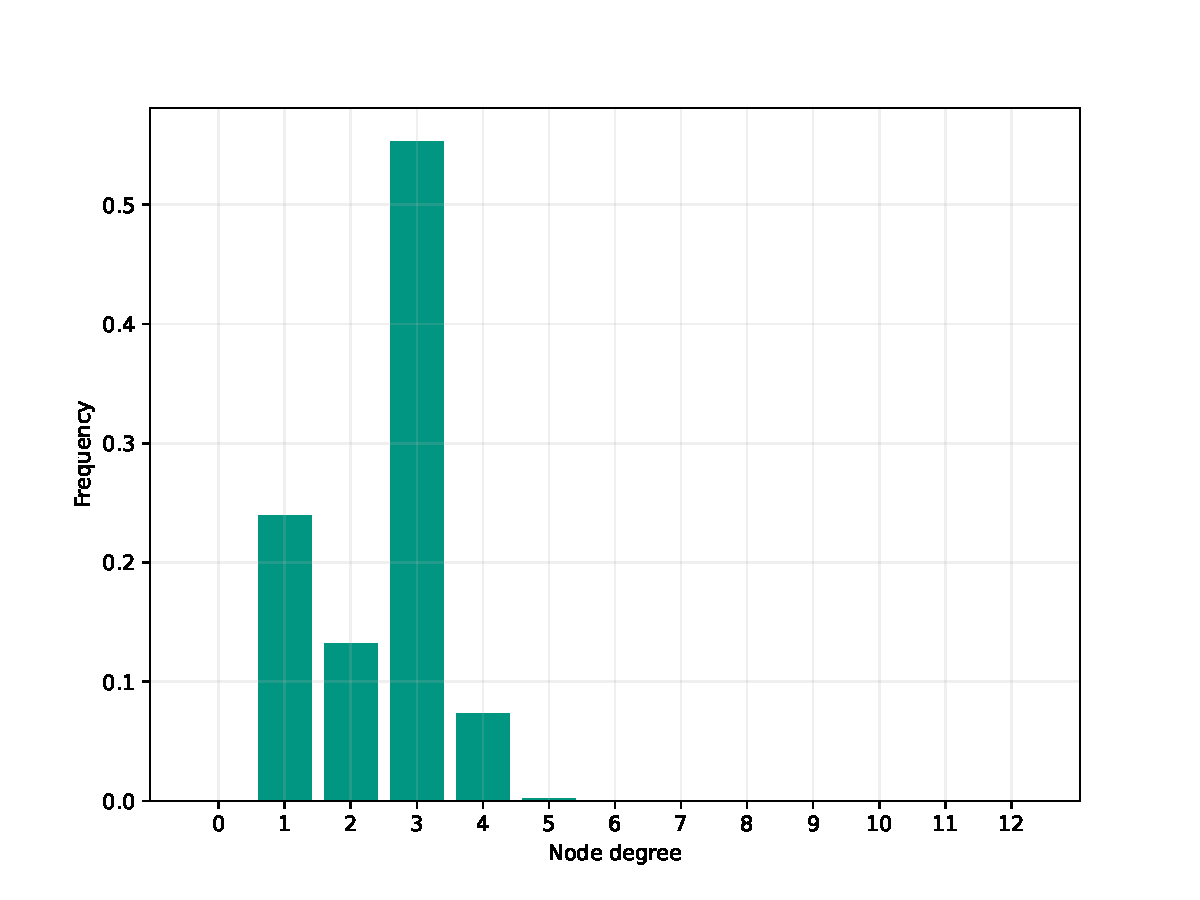
\includegraphics[width=0.6\linewidth]{graphics/degree_overview_europe.pdf}
    \caption{Degree distribution of the PTV Europe road network. The x-axis represents the vertex degree, and the y-axis shows the fraction of vertices with that degree. A single node with degree 12 has the highest degree.}
    \label{fig:degree_dist_europe}
\end{figure}

To examine whether this low average degree alone is sufficient to yield small separators, we generated connected random graphs matching this average degree.
The generation process involved two main steps.
First, a random spanning tree was created for a given set of \(n\) vertices using the algorithm described by Broder \cite{broder_generating_1989}.
This algorithm performs a random walk starting from an arbitrary vertex on the complete graph of \(n\) vertices.
An edge is marked as part of the spanning tree the first time a vertex is discovered via that edge during the walk.
The process continues until all vertices have been visited, resulting in a uniformly sampled random spanning tree in expected time \bigO{n \log n}.

It is noteworthy that random trees generated in this manner exhibit properties distinct from those of road networks.
For instance, the diameter of such random trees is known to be in \bigO{n^{1/2}} \cite{chlamtac_tree-based_1987}.
This contrasts sharply with empirical observations on road networks, such as subgraphs from the nested dissection of the Karlsruhe graph, where the diameter appears significantly smaller, estimated empirically as \bigO{n^{0.3737}}.
This observed diameter growth is visualized in \cref{fig:diameter_karlsruhe}.

\begin{figure}
    \centering
    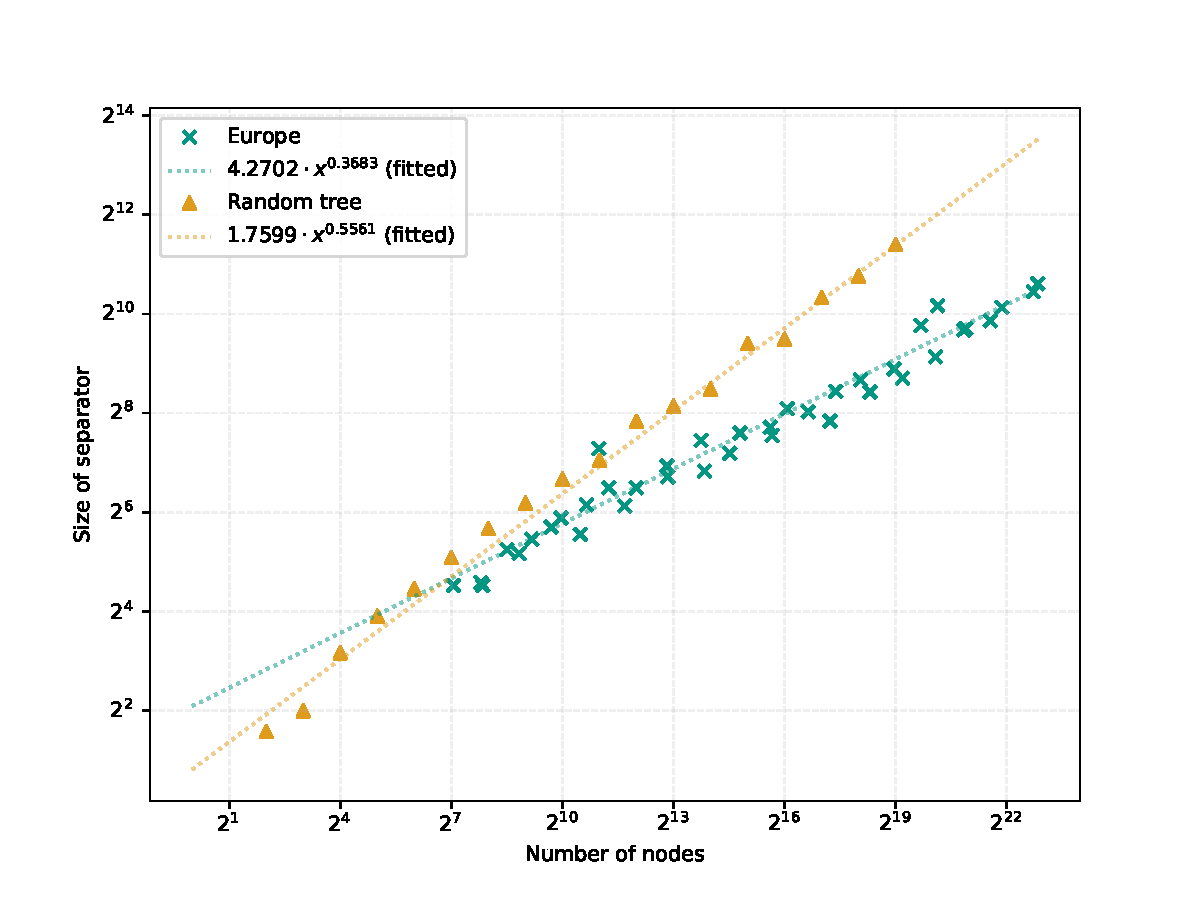
\includegraphics[width=0.6\linewidth]{graphics/diameters.pdf} 
    \caption{Empirical diameter growth observed in the Karlsruhe road network subgraph. The plot shows the diameter (y-axis) as a function of the number of nodes \(n\) (x-axis, log scale).}
    \label{fig:diameter_karlsruhe}
\end{figure}

Following the generation of the initial random spanning tree, we proceeded to the second step: adding edges randomly between pairs of non-adjacent vertices.
This edge addition continued until the target average degree of \(2.47\) was reached for the entire graph.
The resulting graphs, by construction, lack the inherent locality often present in road networks.
A consequence of adding these random edges was a significant decrease in the graph diameter.
For example, graphs generated with one million nodes using this method exhibited diameters of approximately 40.

These synthetic graphs did not replicate the small separator sizes observed in real-world road networks.
Experiments yielded very large separators, with sizes scaling as \bigO{n^2}, as illustrated in \cref{fig:same_degree}.

\begin{figure}
    \centering
    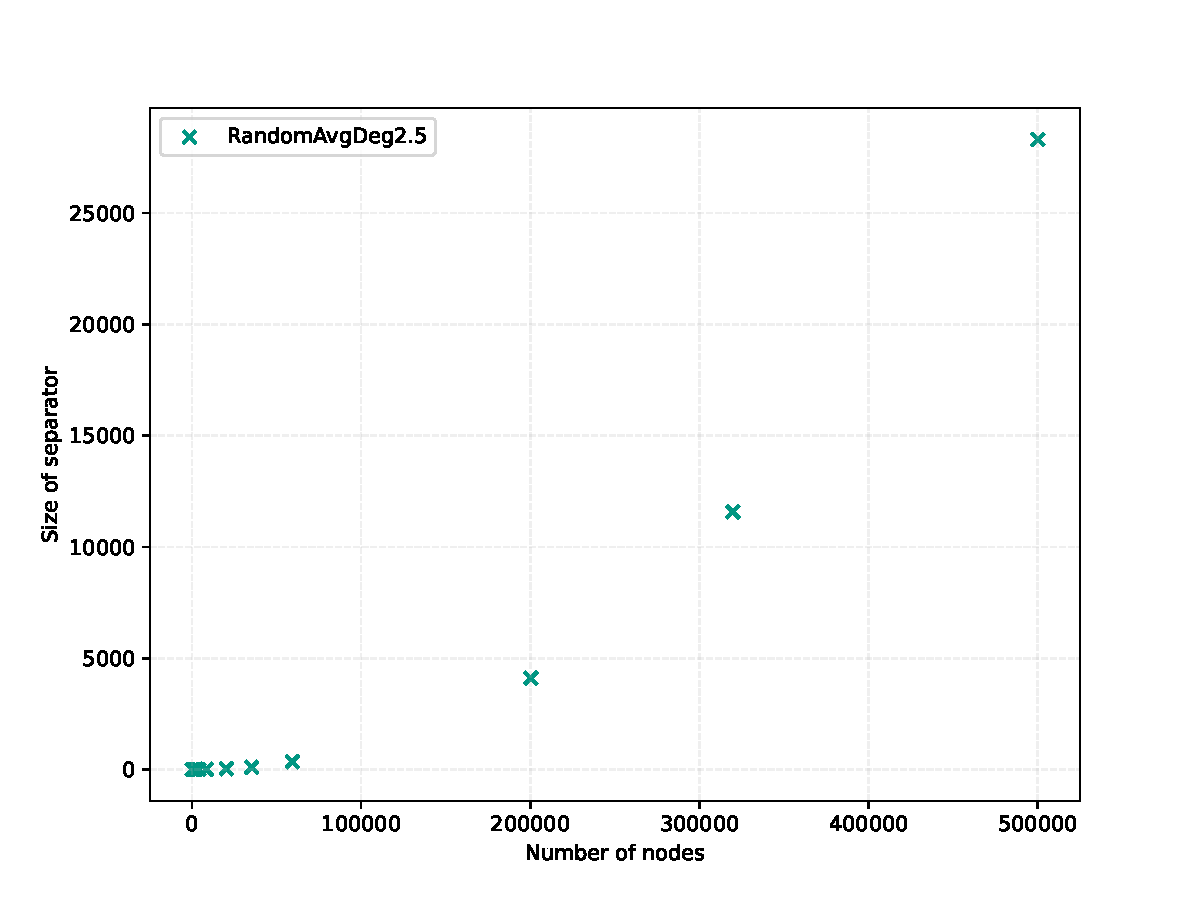
\includegraphics[width=0.6\linewidth]{graphics/RandomAvgDeg2.5.pdf} 
    \caption{Separator sizes observed in synthetic graphs generated with an average degree matching the PTV Europe road network (\( \approx 2.47 \)). The plot shows separator size (y-axis) versus graph size \(n\) (x-axis). The observed separator sizes are significantly larger than those found in actual road networks and scale as \bigO{n^2}.}
    \label{fig:same_degree}
\end{figure}

We also conducted experiments generating graphs that matched not just the average degree, but the specific degree distribution of the reference road network.
This involved a similar process of starting with a random tree and adding edges randomly.
However, edge addition was constrained: an edge \( (u, v) \) was only added if adding it would not cause either vertex \(u\) or \(v\) to exceed the count allocated for their respective degrees according to the target distribution sampled from the road network.
The results obtained from this refined approach were largely similar to those using only the average degree constraint.
The generated graphs continued to exhibit large separators, reinforcing the conclusion drawn from the average-degree matching experiments.

These findings suggest that the degree distribution alone is likely insufficient on its own to explain the empirically observed small separators.
Nevertheless, the low average degree remains an important factor.
Intuitively, sparser graphs, possessing fewer edges overall, should generally be easier to partition compared to denser graphs.
